\begin{figure*}%
	\centering%
	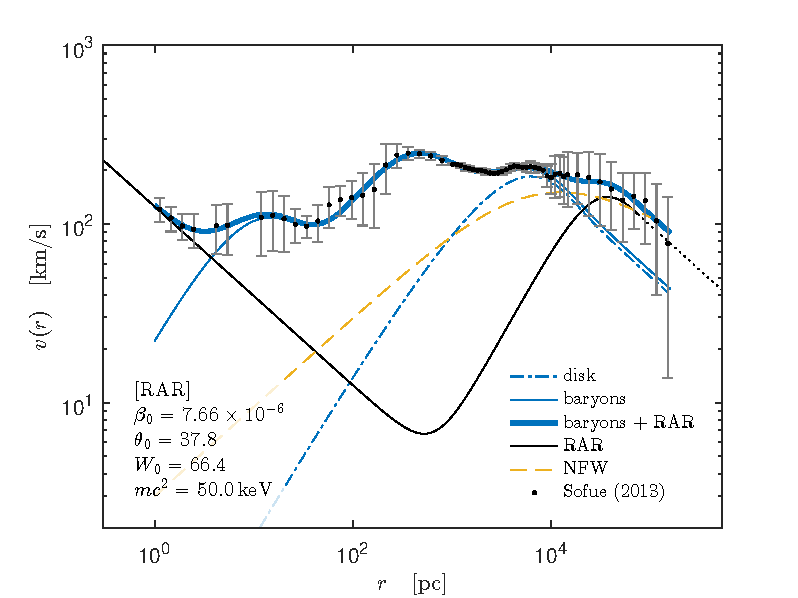
\includegraphics[width=0.5\hsize]{\ROOTPATH/rctotal.pdf}%
	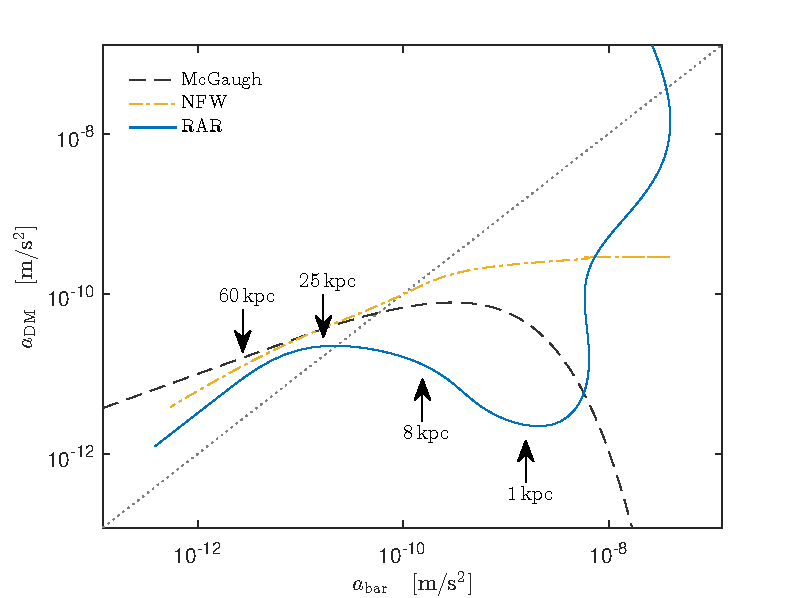
\includegraphics[width=0.5\hsize]{\ROOTPATH/acdark.pdf}%
	\caption{Rotation curves (left) and radial acceleration correlation (right)for the Milky Way galaxy. The observed velocities (black dots with error bars) are compared with the total velocity (thick solid line). The latter is composed of the baryonic component (dashed line), including a disk component (dot-dashed line), and the best-fit of the DM component, modeled with $50\mathrm{keV}$-RAR (thin solid line). For comparison, the NFW profile is added. The radial acceleration correlation from the RAR model (solid line) is compared with McGaugh's empirical fit (dashed line) and the results from NFW model (dot-dashed line). The dotted line describes where the centripetal acceleration of dark and baryonic matter are equal. Thus, in the top-left corner is the dark matter dominated region and in the bottom-right corner is the baryonic matter dominated region. The transition appears at about $2\times 10^{-11} \mathrm{m/s^2}$. In the very high acceleration regime the RAR model predicts an increase of dark matter acceleration due to the degenerate dark matter core in the Galactic center.}%
\label{fig:mw}
\end{figure*}